\chapter{Literature Review and Related Works}
\label{ChapterII}
	
\section{What is Institutional Investment?}
\nomenclature{SEA of 1934}{Securities Exchange Act of 1934}
	
Institutional investors are defined in the Securities Exchange Act of 1934 (henceforth referred to as the SEA of 1934) as investors (natural or legal entities\footnote{Institutional investors can organize under different corporate structures, such as banks, insurance companies, defined benefit pension fund, investor broker-dealer, hedge fund and incorporated company.} ) with investment discretion (or beneficial ownership) over a pool of funds greater than one hundred million dollars\footnote{The statute allows for the Securities and Exchange Commission to lower the threshold to a number no small than ten million dollars.  However, this discretion has not been exercised as the date of publication \citep{Davis2001}.  US Code. Title 15 - Commerce and Trade, Chapter 2B - Securities Exchanges, 78m. Available online at \url{www.law.cornell.edu/uscode/pdf/uscode15/lii_usc_TI_15_CH_2B_SE_78m.pdf}}.  The theory is that by pooling capital, investors are in a better position to manage investment risk, and thus achieve a better risk-adjusted return \citep{Davis2001}.  Those more familiar with the investment literature will see the obvious hand of the efficient frontier hypothesis, in which larger pools of capital can more efficiently manage negatively correlated investment positions \citep{Markowitz1952}.    
	
\subsection{History of Institutional Investment}

\cite{Blume2012} trace the history of institutional investors to the first decade of the twentieth century, where they accounted for approximately five percent of the U.S. stock market and about two thirds of the US Stock market in 2010.  Commenting on this growth, \cite{friedmaneconomic1996} notes that the share of institutional money in the US stock market grew fastest in the decades after the second world war, going from approximately 10 percent in 1950 to just under 50 percent in 1994. Similarly, the Institutional Investor Study by the \cite{U.S.SecuritiesandExchangeCommission1971} found, with a strict definition of institutional ownership of all outstanding stock in the stock-market at seven percent in 1900, and 19 percent in 1952.  Using a broader definition of institutional investor, the study found ownership of 24 percent of outstanding stock in 1952 and 26 percent in 1958.  Regardless of the definition used by the report, institutional ownership favoured positions that invested disproportionately in large publicly traded companies.  Also cited in the congressional report was a census of stock ownership done by the New York Stock Exchange.  This study found institutional ownership of all outstanding stock on its exchange showed growth from 31.1 percent in 1962 to 35.5 percent in 1965 and to 39.4 percent in 1970. 
	
There's a similar growth trend within the subset of institutional investors called hedge funds.  Using their own proprietary research and government supplied data, the research firm BarkleyHedge publicizes a count of hedge funds operating in the universe of US securities.  Figure \ref{fig:hedgefundsundermanagementbarkleyhedge} demonstrates the evolution of hedge fund assets under management from a rapid recovery and growth in assets under management in the early 2000s stock market boom, followed by a precipitous drop after the Great Financial Crisis of 2008, superseded by a slow and steady rise during the Obama recovery.  

\begin{figure}[ht]
	\centering
	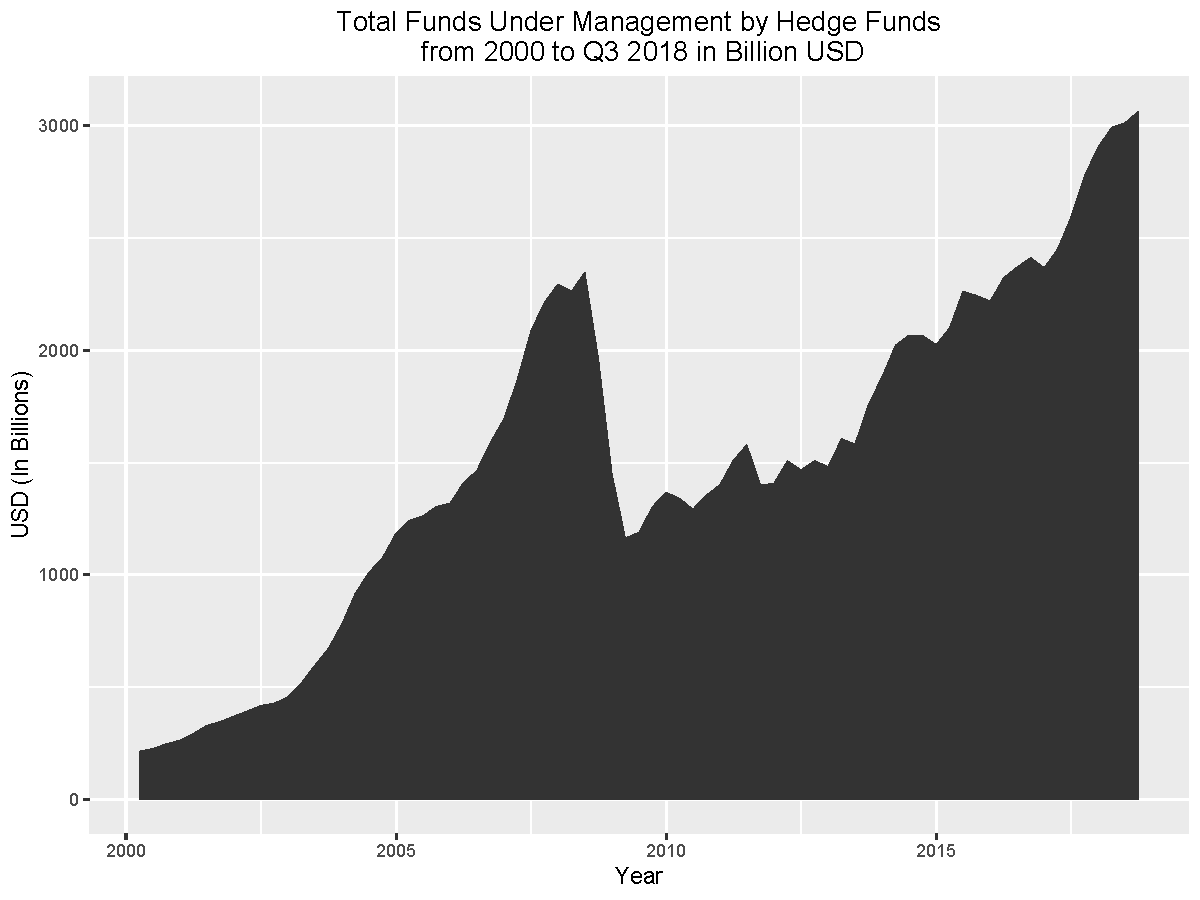
\includegraphics[width=1\textwidth]{Figures/ChapterII/Hedge_Funds_Under_Management_Barkley_Hedge.pdf}
	\caption[Funds Under Management for Hedge Funds from 2000 to Q3 2018]{Total funds under management as measured by the research firm BarkleyHedge in December 2018.}
	\label{fig:hedgefundsundermanagementbarkleyhedge}
\end{figure}
	
\nocite{BarclayHedge2018}
	
Therefore, there's a consilience from these authors showing the gradual rise in importance of institutional investors in the US stock market across the 20th century.   
	
\subsection{Fears and Questions about Institutional Investment in the 1960s}
	
While the definition of investor capitalist can become quite broad -- anybody who engages in market activity for profit can be defined as a capitalist -- most people and institutions of modest means have a marginal impact on the market as a whole. At the other extreme, many fear that the concentration of substantial pools of capital can have a distorting effect on markets in a manner akin to how stellar objects gain influence over their peers via gravity as they accrue mass. To continue with the Newtonian gravity analogy, it was hoped that periodic disclosure of investments by the largest investors would shine a light on their stock movements and thus level the playing field with investors of more modest means. This periodic reporting would chart the distortions caused by large pools of capital, just like how gravitational distortions on other planets were used to predict and find the orbit of the planet Neptune. 
	
The legal mechanism that mandates the periodic disclosure of institutional capital is Section 13F of the SEA of 1934.  This section of law was signed by President Gerald Ford in January of 1975 and took effect in 1978 \footnote{US Code, Title 15, Chapter 2b, 78m}\nocite{US Code}. Yet, the passing of this bill was a long and tortuous affair spread over the better part of a decade and spanned four different congresses as well as the presidencies of Lyndon Banes Johnson and Richard Milhous Nixon. A look at the bill's legislative history, the rational, as well as what was discarded during the sausage-making process of getting legislation passed, can provide insight on what the bill was meant to cover, what it wasn't meant to cover, in addition to the intended use of the tools created by the bill.  
	
During much of the 1960s, there was fear that some shadowy cabal of investors were manipulating the stock market - seen as a key driver of American success in the cold war - to their own ends and to the public's expense via underhanded techniques such as front-running and manipulating who could serve on the board of directors.  In order to allay fears and find remedies if such action were warranted, the 91\textsuperscript{st} Congress (January 3, 1969 to January 3, 1971) commissioned a study which was completed and presented in front of the 92\textsuperscript{nd} Congress \citep{Hearing71}.
	
While the 1971 report could not prove extant manipulation by institutional investors, the report did suggest that a periodic disclosure of investment positions would help allay fears by increasing transparency in the market and thus reduce the perception of corruption. Furthermore, the report shows that investors -- across different lines of investment, be it insurance, banks, pension funds among others -- were increasingly conscious of ``performance" and thus were willing to increase the risk of their portfolio in exchange for higher yields \citep{U.S.SecuritiesandExchangeCommission1971}.  However, the commission found in interviews with investors that they were unaware of the nature of the risk they were running by chasing higher yields. In order to protect investors, the report suggests that periodic disclosure of investment risk would help investors balance risk and reward in their investment decisions and looked for regulatory tools to make this a reality. The report also found that the SEC had the pre-exiting statutory authority to require increased risk reporting for mutual funds under the Investment Company Act of 1940, but that institutional investors were not covered by this Act since by their very nature institutional investors were not a public facing investment provider.  As a consequence, the SEC asked the Congress for tools to mandate regular disclosure of stock holdings for institutional investors.  
\nomenclature{SEC}{Securities and Exchange Commission}
One more problem uncovered by the report was the disparate treatment of domestic and offshore investment funds.  It was found that in practice, funds that operated outside of the territorial jurisdiction of the United States had a competitive advantage since they operated under a more permissive regulatory and taxation regime.  The report suggests that by equalizing the playing-field by forcing foreigners to register with the Securities and Exchange Commission, foreign investors would also receive stronger consumer protections.  
	
Senator Harrison Williams\footnote{Ironically Senator Williams is the only Senator successfully convicted during the ``ABSCAM'' investigation into Congressional corruption in the early 1980s. \cite{gershmanabscam1982}}  (D-NJ) shepherded the 13F amendment through multiple reform minded Congresses \citep{Shaw1981}. 	The first pieces of legislation that can be recognized as the ancestors of the current Section 13F are a pair of bills called Senate Bill 2234 and Senate Bill 2683.   The more ambitious bill (Senate Bill 2234) had a more inclusive definition of who is an institutional investor, a reporting threshold of 10 million dollars rather than 100 million dollars in S.2683, as well as mandating reporting of a broader basket of holdings, such as real estate, art, bonds, cash deposits, and commodities in addition to securities. By contrast, Senate Bill 2683 is the more modest of the two bills that Senator Williams presented concurrently to the Senate Banking committee and is substantially similar to the present section 13F of the Securities and Exchanges Act of 1934 \citep{Hearing71}. 
	
Senate Bill 2234 was deemed to be too invasive and impractical by the ranking member Bill Bennett (R-UT) since the broader basket of disclosure wasn't as easily priced as securities that are openly and regularly traded on various exchanges.  As a compromise, language was added to Senate Bill 2683 to give the SEC discretion to ratchet down the reporting threshold to 10 million dollar should they feel it necessary \citep{Hearing71}. 
	
Senate Bill 2683 sailed out of the banking committee and passed in the Senate with little opposition.  However, the bill did not make it to the House of Representatives.  Journalists covering this story attribute the failure in the lower house to the intrepid lobbying by Wall Street agents upset by the lowering of brokerage rates that was recommended by the Congressional report \citep{Zimmerman1971}.  During the lame duck session between the 93\textsuperscript{rd} and  94\textsuperscript{th} Congresses, Senator Harrison Williams went on a publicity tour in order to drum up support for the bill in the face of the New York based opposition \citep{Dallos74,Dallos74a}.  His efforts were rewarded when the language to create section 13F of the SEA of 1934 was passed by Congress early in the 94{th} Congress and was signed into law by President Gerald Ford on June 4\textsuperscript{th}, 1975 \citep{libraryofcongress}. 
	
\section{Why Geography and not Economics}
	
\subsection{Trading in Aspatial Random Walks}
	
\nocite{Bachelier1900} 
In 1900, French mathematician Louis Bachellier submitted his thesis called \textit{"Th\'{e}orie de Sp\'{e}culation"}, in which Bachellier formulated that the long-run expected value of speculation on a market experiencing a random walk process was zero. In other words, if one were to assume that the stock market was truly random and thus had a long term trend of zero, it would be impossible to gain money off the stock market by buying and selling stocks only at the opportune time over a sufficiently long time period. While the mathematical proofs in Bachellier's work was more intuitive than rigorous, often hinting mathematical concepts that would shape the field of Mathematics in the twentieth century such as Brownian motion and Markov chains, this work was an important stepping stone to Eugene Fama's Efficient Market Hypothesis \citep{Courtault2000}. 
	
\nomenclature{EMH}{Efficient Market Hypothesis}
The Efficient Market Hypothesis (EMH) \citep{Fama1970,Fama1991} posits that asset prices fully reflect all available information.  As such, it follows that it's impossible for the average investor to continuously outperform the market average performance on a risk adjusted basis since any information is updated and baked-into the price of the security. Eugene Fama offers the theory in three related variants: Weak, Semi-Strong, and Strong. The Weak variant posits that it is impossible to derive future prices from past information, the Semi-Strong variant posits that current prices reflect all known public information and the Strong version that all information (private and public) is reflected in the price \citep{Fama1970}.  \cite{Graves2003} argues that this seminal paper cast a long shadow on the field of investment research, to the point that many papers fail to consider geography as a plausible explanation for sustained trading advantage, since it would violate the Semi-Strong and Strong version of the EMH. For example, \cite{Easley2011} find that hedge funds survive on information asymmetry, private knowledge and price ambiguity, but fail to inquire about possible sources for these sustained advantages.  Similarly, \cite{Cohen2008} find that mutual funds overweight stocks of firms in which the directors of the mutual funds have a board of directors connection with a shared educational network (\textit{alma matter}), but fail to consider current social networks and geographical proximity as confounding variables.	
	
That being said, the literature is rife with studies that appear to conciliate on the point that there is some geographic bias in investment returns and that these abnormal returns stem mostly from local information asymmetry. However, it does appear that this phenomenon was stronger prior to the information technology and telecommunications revolution that was ushered in during the 1980s.  
	
\subsection{Big Role for Geography} 
	
From the first market towns to Marshallian industrial districts, commerce and other economic activities are the \textit{sine qua non} of its existence. An inherent advantage of being located at a trade nexus is the ability to easily compile information on market conditions. \cite{Westaway1974} finds that as firms grow, management functions aggregate towards larger urban centres since these places have greater access to necessary specialized information.  This serves as a foundation for \cite{pred1977}, where they theorizes that the location of information-intensive activities is a positive feedback process. Furthermore, \cite{JAMES1988} as well as \cite{WheelerMitchelson89,Wheeler1989} show that urban centres see benefits proportional to their relative importance in corporate decision making.  This fits nicely with Quaternary Location Theory (QLT)\citep{Semple85}\nomenclature{QLT}{Quaternary Location Theory} which emphasises that command and control functions will naturally aggregate to large urban centres.
	
While the initial flurry of Quaternary Location Theory papers focused mostly on corporate locational preferences -- specifically command and control centres, it wasn't long before the field turned its attention towards banking and investment. An early paper \citep{greena1993} looked at the geography of institutional investment.  This paper looks at inter-city ownership of American institutional investors by using a sample of 395 institutional investors that held stocks in Fortune 500 companies for the year 1980.  In this sample, New York City is the only city in the first tier of urban hierarchy, followed by a set of four second tier cities and a steep decline thereafter.  The ranking in between city population and financial ownership is not correlated and the ordinary least-squares (OLS) spatial gravity model explains about 6 to 9 percent of the local bias in holdings.  In a follow-up paper \citep{Green1995} the author adds an additional time window (1990) and compares the new data with the data from 1980.  The OLS spatial gravity model for 1990 is quite different than the model for 1980, showing a more diffused spatial process, which the author ascribes to the increased role of telecommunications.  Green also notes the absolute increase of investors in New York City, but that its role is less dominant in the urban hierarchy in 1990 than it was in 1980.  
	
\cite{GreenMeyer1996} examines the spatial distribution of mutual funds from 1940 to 1985.  They find that most mutual funds are managed out of 3 main cities: New York, Boston and Chicago (in that order).  Using log-linear analysis on three explanatory variables (location  tier \footnote{Core, Semi-Core and Periphery}, year and mutual fund type), the researchers find that they can rule out a 3 way interaction, but can't rule out a 2-way interaction in the data.  Closer examination shows that the most profitable funds are located in core cities.  
	
\cite{gravesthe1998} examines the location of mutual fund companies for the year 1996. The author posits that the size of a fund is a function of the fund's past performance, and that the past performance is somewhat dependant on the amount and quality of information available. 
	
\cite{gravesthe1998} gives three reasons why mutual funds have different spatial patterns than banks.  The first reason is that mutual funds and banks have a different history of spatially-based regulations.  More specifically, mutual funds did not experience the State banking era regulatory regime.  Secondly, unlike banks which need to interact with customers on a regular basis to perform banking functions such as check cashing and bill payment, mutual funds can conduct their business by mail and other methods of communication.  Lastly, banks and mutual funds have different economies/diseconomies of scale curves with regards to personnel and investment positions.  This is mostly due to the fact that investment positions do not scale well, as they become more illiquid with size.  
	
While \cite{gravesthe1998} hypothesizes that the control nexus of investment funds will coalesce into the cities at the top of the urban hierarchy, the opposite seems to be happening, for smaller centres are growing faster than larger cities.  A possible explanation for drop in the growth rate of funds in New York City is that modern telecommunications have reduced benefit of co-location to the point that the higher rent is no longer commensurate with the locational advantage. According to Graves, this result calls into question the ability of Quaternary Location Theory to explain the contemporary pattern of investment locations. Graves offers as an explanation that the theory was written during an era with highly aggregated data and inferior communications technology -- lacking fax, internet and low cost wireless communication.     
	
Outside of Geography and located mainly in Finance and Business, there exists a parallel literature examining the influence of locational choice and investment returns. Furthermore, this literature is highly steeped in empirical examinations over fitting evidence into established geographical theories. \cite{Hau2001} finds that traders on the Frankfurt Stock Exchange who are located in Frankfurt outperform traders located outside of Frankfurt on a intra-day basis, suggesting that there is an information distance decay function.  Similarly, \cite{Dovak2005} reports that foreign traders fare worse than domestic traders at the Jakarta stock exchange, and	\cite{choedo2004} discover that foreign-born traders pay on average 21 basis points more than domestic traders when buying stocks, and received 16 basis points less than domestic traders when selling. Meanwhile, \cite{teothe2009} found that hedge funds with offices in the same country as their investments outperform hedge funds without an office in the same country as their investment. 
	
Following this trend,  \cite{Zhu2002} used data from a discount brokerage firm and found that individual investors show a propensity to invest in companies that are local to them, and that this propensity cannot be explained by fundamentals-based investment strategies.  Since these individual investors are also more likely to invest in firms that advertise heavily, the author suggests that this is a results of investors being biased by firms they find familiar.  This finding is similar to the findings of \cite{Huberman2001}, who found that owners of Regional Bell Operating Companies tend to live in areas that were served by the company.  That being said, \cite{Monk2009} states that while investing in firms in which the investor has a high level of familiarity may represent a sub-optimal strategy from the point of view of traditional portfolio theory. In some cases, it can provide for those willing to look beyond the efficient market hypothesis a source of information overlooked by the market and thus a way to profit from information asymmetry. That being said, well publicised investment flops in which State pension funds are used to prop-up failing local champions leading to large losses, such as the 80 percent haircut the State of Connecticut experienced on its loan to Colt Industries in the early 1990s, can make this type of strategy politically difficult to execute. 
	
\cite{Bradley2016} report that, in a sample of 16 internally managed state pension funds, they are over-weighted in local companies by 26 percent relative to the average portfolio.  Furthermore, these investments occur predominately in companies that are active in local politics, as measured by both political donations and active lobbying.  The authors explore three non-mutually exclusive explanations for this over-investment: 
\begin{enumerate}
	\item \textbf{Information advantages due to local effect:}  This theory posits that political connections lead to better information flow to the pension fund trustees, and this can be used for trading advantage.
	\item  \textbf{Familiarity:}  This theory posits that managers are more familiar with local firms and over-estimate the quality of their information, but is otherwise a neutral position.
	\item \textbf{Pay to Play:}  This theory posits that political bias and influence peddling leads to malinvestment of State pension funds into politically connected firms.  These conflicted motives lead to worse performance. 
\end{enumerate}
In total, the evidence (that the effect is stronger in States with a larger share of politically appointed pension fund board trustees as well as States with more powerful members of congress) points towards solution 3 as being the most likely.  
	
\cite{malloythe2005} reports that geographically proximate analysts outperform distant analysts in their buy and sell recommendations. The author posits that analysts who make house calls rather than conference calls can obtain more valuable and actionable private information via face to face communication, direct view of the operations floor, talk to floor employees as well as being better positioned to talk to suppliers.  The effect is stronger in smaller locals.  Similarly, \cite{Farooq2013} studied the buy and sell recommendations by foreign and local stock analysis covering Thailand, Indonesia, Malaysia and South Korea during the Asian Financial crisis (1997-1999).  This study found that foreign-based analysts had more accurate buy recommendations, whereas local analysts had more accurate sell recommendations.  Furthermore, \cite{Eckel2011} found, via spatial regression analysis, larger returns than what would be expected for investment firms that invested in companies within a headquarter with 50 miles of their location compared to a random portfolio of companies with similar attributes.  
	
Continuing on the theme of information decaying over distance providing real investment advantages,	\cite{Cashman2017} use the cost of borrowing capital for publicly traded real estate companies in Asia-Pacific as a proxy for the cost of information opacity. The authors conclude that more diffused firms (those operating in more than one country) have higher capital costs than firms that only operate in one country and thus they posit that companies pay an opacity tax.   

In an interesting parallel to the debate on the importance of Marshallian agglomeration with regards to footloose industries, that is to say those that do not necessitate large fixed upfront costs such as factories, \cite{Mitchell_London_2019} looks at the productivity of literary authors of the 18\textsuperscript{th} and 19\textsuperscript{th} century. This study found that when controlling for a multitude of factors authors were most productive when located in London UK and that there's a statistically robust relationship between time spent in London and increased productivity.  Furthermore, the results of this paper suggest that there was a benefit to being located in London that was not present in other UK and Irish literary cities such as Edinburgh or Dublin.  The paper posits that geographic concentration fosters thicker social networks with their peers, individuals of influence (agents, editors, publishers) and patrons, thus facilitating the ease of getting published. 	
\nomenclature{OLS}{ordinary least squares}
	
\subsection{Moderate Role for Geography}
	
There exists other literature that believe that locational advantages were quite measurable prior to the telecommunications revolution of the 1970s and 1980s, and accept limited role at best for locational advantages to accrue in the face of modern telecommunications technology.
	
During the time period between 1925 and 1978, \cite{rhoades1982size} looked at the distribution of deposits in commercial banks and found that due to bank consolidation that were mostly driven by mergers and acquisitions, the distribution of bank deposits were increasingly concentrated towards the top end of the top 100 largest banks list. Furthermore, while this period saw important demographic changes in the USA with the increasing population in the Southern and South-Western United States, changes in the location of the top 100 largest banks were less reflective of the demographic shift than would be expected in a naive model in which bank size is a function of population.  This suggests that large urban centres with preexisting banking infrastructure have an innate pull factor that make banks less footloose than would otherwise be assumed.  
	

With a more expansive look at locational preferences, \cite{bodenmanthe1998} examines the exodus of  Finance, Insurance and Real Estate (FIRE)\nomenclature{FIRE}{Finance, Insurance and Real Estate} sector firms in downtown Philadelphia, Pennsylvania.   During the period between 1983 and 1993, the concentration of FIRE firms located in downtown Central Business District (CBD)\nomenclature{CBD}{Central Business District} fell from 61.9 percent to 24.9 percent.  Examining why firms were leaving the Central Business District, the author asked FIRE sector businesses for factors that were at the heart of the locational preferences.  Personal preference and quality of life were given as top answers, whereas access to information was not given as a priority.  In a related study, \cite{bodenmanfirm2000} looks at how the information technology revolution permits institutional investors broader choice of location without sacrificing access to high quality and quantity of data/information.  Bodenman finds that not all actions taken by institutional investors require face to face contact, such as accounting and regulatory compliance, portfolio management, and trading.  In contrast, activities that do require face to face contact, such as finding and/or managing clients as well as researching investment opportunities do not require a constant downtown presence. As a consequence, \cite{bodenmanfirm2000} posits that active traders will have a propensity to locate in the CBD, whereas passive investors and quantitative traders will locate in suburban office parks where rent is less expensive.  
	
\cite{gongthe2012} examine the geographical dispersion and return on the island of Manhattan shortly before and in the aftermath of the 9/11 terrorist attack. Of the 79 firms surveyed, fifty-four did not change location, while ten moved on a temporary basis (one month to a year and a half), and fifteen changed locations permanently.  Of the ten who changed locations toward the periphery of the New York area, the most common reason for returning to Manhattan is the ability to meet with clients.  Most of the firms that moved were located in Downtown and Midtown, in contrast,  those that returned were located exclusively in Downtown Manhattan. Furthermore, the survey says that prior to the 9/11 attack, most firm managers were reporting that their locational preferences were shaped by maximising the prestige of the building, adjacency to the New York Subway system, as well as being conveniently located in order to meet with clients.    After the attack, the location preference was dominated by an emphasis on office space, building infrastructure and rental costs, while keeping in mind that high prestige buildings would be more susceptible to terrorism in the future.  
	
And while we may not have seen the death of distance as predicted by \cite{Obrian1992}, it can be argued that there is a role for space and place, as well as telecommunications reducing the benefits of co-location. This is the heart of the paper by \cite{Moriset2009} where they argue that modern telecommunications re-arrange spatial forces of agglomeration.  Better communications reduces the need for vertical hierarchies and remove the premiums of co-location. 
	
	
	
	